\documentclass[a4paper,12pt]{report}

\usepackage{microtype}
\usepackage[utf8]{inputenc}
\usepackage[dvipsnames]{xcolor}
\usepackage{listings}
\usepackage{url}
\usepackage{minted}
\usepackage[numbers]{natbib}
\usepackage{graphicx}
\usepackage{wrapfig}
\usepackage{float}
\usepackage{csquotes}
\usepackage{textcomp}
\usepackage{dirtree}
\usepackage{subcaption}
\usepackage{setspace}
\usepackage{verbatim}
\usepackage{siunitx}
\usepackage{float}
\usepackage{lmodern}
\usepackage{url}
\usepackage{color}

\definecolor{lightgray}{gray}{0.94}

\lstset{
    showstringspaces=false,
    basicstyle=\ttfamily,
    keywordstyle=\color{blue},
    commentstyle=\color[grey]{0.6},
    stringstyle=\color[RGB]{255,150,75}
}


\lstdefinelanguage{kotlin}{
  keywords={package, as, typealias, this, super, val, var, fun, for, null, true, false, is, in, 
throw, return, break, continue, object, if, try, else, while, do, when, yield, typeof, yield, 
typeof, class, interface, enum, object, override, public, private, get, set, import, abstract, },
  keywordstyle=\color{NavyBlue}\bfseries,
  ndkeywords={@Deprecated, Iterable, Int, Integer, Float, Double, String, Runnable, dynamic},
  ndkeywordstyle=\color{BurntOrange}\bfseries,
  emph={println, return@, forEach,},
  emphstyle={\color{OrangeRed}},
  identifierstyle=\color{black},
  sensitive=true,
  commentstyle=\color{gray}\ttfamily,
  comment=[l]{//},
  morecomment=[s]{/*}{*/},
  stringstyle=\color{ForestGreen}\ttfamily,
  morestring=[b]",
  morestring=[s]{"""*}{*"""},
}

\newcommand{\inlinecode}[2]{\colorbox{lightgray}{\lstinline[language=#1]$#2$}}

\newcommand{\scalainline}[1]{\inlinecode{scala}{#1}}
\newcommand{\ktinline}[1]{\inlinecode{kotlin}{#1}}

\AtBeginEnvironment{minted}{
  \renewcommand{\fcolorbox}[4][]{#4}
}


\renewcommand{\bibname}{References} % so that the table of contents updates too
\usepackage{tocbibind}
\usepackage[hidelinks]{hyperref}

% Title Page

\begin{document}

\begin{titlepage}

\newcommand{\HRule}{\rule{\linewidth}{0.5mm}}

\center % Center everything on the page
 
%-------------------------------------------------------------------------------
%   HEADING SECTIONS
%-------------------------------------------------------------------------------

\textsc{\LARGE École Polytechnique Fédérale de Lausanne}\\[1.5cm]
\textsc{\Large Master Semester Project}\\[0.5cm]
\textsc{}\\[0.5cm] % Minor heading such as course title

%-------------------------------------------------------------------------------
%   TITLE SECTION
%-------------------------------------------------------------------------------


\HRule \\[0.4cm]
\begin{spacing}{2}
{\huge \bfseries Production-level tooling for the Kotlin to Scala.js compiler}
\end{spacing}
%\vspace{-10pt}\\[0.4cm] 
\HRule \\[1.5cm]
 
%-------------------------------------------------------------------------------
%   AUTHOR SECTION
%-------------------------------------------------------------------------------

\begin{minipage}{0.4\textwidth}
  \begin{flushleft} \large
  \emph{Author:}\\
  Florian \textsc{Alonso} % Your name
  \bigskip \bigskip \bigskip \bigskip
  \end{flushleft}
\end{minipage}
~
\begin{minipage}{0.4\textwidth}
  \begin{flushright} \large
  \emph{Professor:}\\
  Martin \textsc{Odersky}\\
  \bigskip
  \emph{Supervisor:} \\
  Sébastien \textsc{Doeraene} % Supervisor's Name
  \end{flushright}
\end{minipage}\\[2cm]

% If you don't want a supervisor, uncomment the two lines below and remove the 
%section above
%\Large \emph{Author:}\\
%John \textsc{Smith}\\[3cm] % Your name

%-------------------------------------------------------------------------------
%   DATE SECTION
%-------------------------------------------------------------------------------

{\large \today}\\[0.5cm]
{\large LAMP}\\[1cm]

%-------------------------------------------------------------------------------
%   LOGO SECTION
%-------------------------------------------------------------------------------

\begin{figure}[b]
    \centering
    \begin{subfigure}[b]{0.30\textwidth}
      \flushleft
        
      
\includegraphics[width=\textwidth]{imgs/epfl_logo.png}\\[1cm]
    \end{subfigure}
\end{figure}
 
%-------------------------------------------------------------------------------

\vfill % Fill the rest of the page with whitespace

\end{titlepage}

%\include{abstract}

\chapter*{Acknowledgements}
% required to add entry without any numbering
\addcontentsline{toc}{chapter}{Acknowledgements}

\paragraph{} I would like to thank my advisor, M. Sébastien Doeraene, for all the support he provided me with and for the advice he gave me during this semester of work. His help has been very valuable to me and has allowed me to learn many things along the way.

\paragraph{} A huge thank you to my friend Dennis as well, who helped me find inconsistencies in this report by reading through it in time of exams.

\paragraph{} Thank you finally to the EPFL and LAMP for giving me the opportunity to work on this project.

\tableofcontents

\chapter{Introduction}
\section{Kotlin and Scala.js}

\paragraph{} JavaScript (JS for short) is a programming language that provides developers with a 
way to interact with users by building dynamic web applications and websites. Through the use of 
JavaScript runtimes, such as Node.js~\cite{nodejs}, it is no longer required that applications be 
executed only on the client side. It can therefore also be used to build a large range of 
server applications. Many frameworks and libraries exist to provide useful functionalities to the 
language and ease the development of said applications.

\paragraph{} JavaScript is a weakly typed  language and provides a large freedom on how to organize
one's code. However, depending on the situation, a strongly typed language might be more suitable for development. This is where Kotlin JS and Scala.js come into play.

\paragraph{Kotlin JS} Kotlin~\cite{kotlin} is a statically typed programming language providing 
many features through its large standard library. It is able to run on the JVM and is officially 
supported for Android since May 2017~\cite{android_kotlin_support}. In order to expand their reach, 
the Kotlin team has built a JavaScript compiler to translate the Kotlin standard library 
and the language capabilities into a JS application. It however lacks some optimizations and 
produces a rather large amount of JS code.

\paragraph{Scala.js} Scala.js~\cite{scalajs} is another typed programming language. Being 
implemented as a Scala compiler plugin, it benefits from most of its features with a few 
differences due to the JavaScript semantics (more details about this can be found in the 
\enquote{Hands on Scala.js} tutorial~\cite{scalajs_handson}).

\paragraph{} Both languages provide specific language features in order to allow developers to interact with 
pre-existing JavaScript objects and thereby provide JavaScript interoperability. The main 
difference between Kotlin JS and Scala.js is the number of optimizations performed on the code before 
outputting JavaScript. The sizes of the final JS files are also very different. 

\paragraph{} Scala.js (mainly thanks to its linker) enhances the performance by performing whole 
program optimizations and greatly reduces the size of the generated code. All details about the 
Scala.js compilation pipeline (and how it optimizes JavaScript code) can be found under section 
\enquote{The compilation pipeline} of the \enquote{Hands on Scala.js}~\cite{scalajs_handson} 
tutorial. Kotlin, since its version 1.1.4, provides Dead Code Elimination through an additional 
Gradle plugin which can be found in the Kotlin documentation~\cite{kotlin_dce}.


\paragraph{} As a summary, combining both the Kotlin language flexibility and the Scala.js 
optimizing capabilities can result in a great improvement for JavaScript applications development 
both in terms of executable size and performance.

\section{Motivations}
\paragraph{} I have always been strongly interested in web related technologies and the 
opportunity to work at the core of one of them is really an enriching experience. The Kotlin 
compiler is a very large code base and having to search trough its numerous source files in order 
to understand the logic behind the language is challenging and at the same time captivating.

\paragraph{} Besides the performance aspect behind the compilation pipeline (and of course the 
language syntax), one of the most important things for a language to be adopted is the tooling 
available and how easy it is to setup a new project and compile one's code.
    
\paragraph{} The main goal of this project was thus to provide developers with basic 
tooling and support for the Kotlin language. This will be achieved by continuing prior work to 
compile the Kotlin standard library to the Scala.js IR and by writing a simple Gradle~\cite{gradle} 
plugin.

\section{Project structure and architecture}

\paragraph{} The work on a Kotlin to Scala.js compiler was started in February 2017 by Lionel 
Fleury and Guillaume Tournigand. Their work resulted in a structured code base which allowed simple 
Kotlin programs to compile (for more details on their work, please refer to their semester project 
report~\cite{kotlin_scalajs_report}). A brief review of the working features of their project is 
available under section \ref{initial_status}.

\subsection*{Main source code}

\paragraph{} The main code of the project is stored under the \scalainline{ch.epfl.k2sjsir} 
(root) package, organized in three subpackages: \scalainline{lower}, \scalainline{translate} and 
\scalainline{utils}.

\paragraph{} More details about this design and the underlying Kotlin AST (PSI, Descriptors and 
Contexts) can be found under section \enquote{Kotlin} of Guillaume's and Lionel's 
report~\cite{kotlin_scalajs_report}.

\paragraph{Package root} A few files are located at the root of the \scalainline{ch.epfl.k2sjsir} 
package and they are the entry point into the Kotlin compiler pipeline. For reference, the 
\scalainline{translate} package is first called via the \scalainline{GenClass} class from the 
\scalainline{PackageDeclarationTranslator} file.
      
\paragraph{Package \scalainline{lower}} This package contains all the logic related to class 
lowering which is used to retrieve inner classes and objects (besides anonymous objects, see 
section \ref{anonymous_objects}) from the Kotlin AST.

\paragraph{Package \scalainline{translate}} This is where the main translation logic is kept. 
It is organized in a generator pattern and thus every class in this package must provide a way to 
retrieve an SJSIR object (generally through a \scalainline{tree} method) from a \ktinline{KtElement}. 
For example if you are provided with a \scalainline{KtExpression} object, you can translate it with:

\begin{minted}[linenos,frame=leftline]{scala}
  val e: KtExpression = /* Retrieve a KtExpression */
  GenExpr(e).tree // This will return a Scala.js IR node
\end{minted}


\paragraph{Package \scalainline{utils}} This last package contains a variety of utility 
methods such as implicit classes which provide an interface to encode names, retrieve types or 
generate recurring SJSIR objects, etc.

\subsection*{Tests}
\paragraph{} In order to verify that no code change breaks the translation of other elements, a 
test suite exists under the \scalainline{test} directory. This directory is organized in two main 
folders which are \scalainline{resources} and \scalainline{scala}.

\paragraph{Folder \scalainline{resources}} There are mainly two directories in this folder; the 
first one, \scalainline{lib}, contains the Scala.js library jar file. These are used when launching 
the Scala.js linker to compile the SJSIR files output by the compiler. The second folder is the 
\scalainline{src} folder which contains all Kotlin sources to test the good behavior of the 
Kotlin to Scala.js compiler.

\paragraph{Folder \scalainline{scala}} It contains the various ScalaTest~\cite{scala_test} files 
which define the unit tests. Each test file was written to test a specific language feature, 
please refer to section \ref{features} for details about which Kotlin feature these test files are 
related to. The corresponding source code can be found in the GitHub 
repository~\cite{kotlin_scalajs_v2}.

\subsection*{General design of the project}

\paragraph{Entry point} The \scalainline{K2SJSIRCompiler} class is used in order to inject the 
Scala.js IR translation logic into the Kotlin compiler. It is where the parsing of the 
command line arguments happens, through the use of the \scalainline{K2SJSIRCompilerArguments} class. The 
resolution of source file paths is then handed to the \scalainline{K2SJSIRTranslator} which in turn 
will delegate the work to the \scalainline{Translation} class.

\paragraph{} Finally, this class will hand the task of generating SJSIR nodes to the
\scalainline{PackageDeclarationTranslator} class. It then makes use of the content of the
\scalainline{translate} package in order to generate the final SJSIR files.

\paragraph{} Since this code is (mostly) a Scala translation of the original  
\scalainline{K2JSCompiler} class, all phases (parsing, type checking, etc.) of the original 
compiler are still there.

%% Compiler pipeline illustration

\label{translation}
\paragraph{Translation} As explained above, the translation happens mainly inside the 
\scalainline{PackageDeclarationTranslator} class. It will extract the various declarations using 
lowering and generate the corresponding SJSIR files. The declarations can be either classes and
objects or top-level functions and properties.

\paragraph{} The reasoning behind this design is explained in more details in the \enquote{Hello 
World} section of Guillaume and Lionel's report~\cite{kotlin_scalajs_report}.

\begin{comment}
  - talk about kotlin representation ?
  - project organization (folders) --> README ?
  - general design of the compiler
  - supported kotlin + scalajs versions
  Annexes
  - brief explanation of the various utils available
  - definition of dispatch receiver, extension receiver
  - kotlin standard library compilation (which files and how)
\end{comment}

\chapter{Supported features} \label{features}
\section{Prior work} \label{initial_status}
  
\paragraph{} This section aims to list the features supported by the prior version of the 
compiler~\cite{kotlin_scalajs_v1} (as of July 2017). This version was built to work with 
Scala.js 0.6.15 and Kotlin JS 1.1.1. Since then, it was upgraded to Scala.js 1.0.0-M2 and Kotlin 
1.1.61~\cite{kotlin_version}.

\paragraph{} Below is a list of all features that were already working (or after minor fixing) on 
the version of the compiler this project started with. For specific syntax examples please refer to 
the Kotlin documentations available online~\cite{kotlin_docs}.

\paragraph{Top-level and extension functions} These are translated the way Kotlin does it. This 
means these definitions are stored in a class named after their containing source file. Top-level 
properties on the other hand are not supported yet.

\paragraph{} For example, if a function \ktinline{fun dummyFun() = println("Hello World")} is 
in a source file called \ktinline{HelloWorld.kt}, it will be stored in a class called 
\ktinline{HelloWorldKt} as a \ktinline{static} definition which is in turn stored in an SJSIR file.

\paragraph{Classes and inheritance} \enquote{Classic} classes  (as opposed to \ktinline{data}, 
\ktinline{enum}, \ktinline{annotation}, etc.) are well supported. They can be declared
(and instantiated) with :

\begin{itemize}
 \item A primary constructor and zero or more secondary constructors.
 \item Inheritance from a superclass (if the class is marked as \ktinline{open}).
 \item One or more \ktinline{init} blocks.
 \item Methods and properties (overridden or not); for properties you couldn't define custom 
getters and setters. However the default ones were generated properly, see section 
\ref{accessor_gen}.
 \item Access to the current class properties and methods. You couldn't however use 
\ktinline{this} nor \ktinline{super} (see sections \ref{this} and \ref{super_calls}).
\end{itemize}

\paragraph{} In the case of \ktinline{inner} classes, the behavior is the same as for nested 
classes. That is, calls to methods and properties of the enclosing class are not supported yet.

\paragraph{} Classes are stored within an SJSIR file with the same name as the class itself. For 
example \ktinline{class Customer} would be stored in file \ktinline{Customer.sjsir}.

\paragraph{Objects} \label{objects}Objects and companion objects are supported at the same level as 
classes. The major difference being that they are generated as module classes (in the Scala.js 
meaning). Their SJSIR file will be named either after the object itself, prefixed with the enclosing 
class name and suffixed with a \$. For example \ktinline{object MyObject} would be written to 
\scalainline{MyObject\$.sjsir} and the following object declaration inside \ktinline{MyClass} would 
be contained in a file named \ktinline{MyClass\$MyCompanion\$.sjsir} as shown in figure 
\ref{companion_example}.

\begin{figure}[h]
\begin{minted}[linenos,frame=leftline]{kotlin}
 class MyClass {
   companion object MyCompanion {
   }
 }
\end{minted}
  \caption{A companion object defined in Kotlin}
  \label{companion_example}
\end{figure}

\paragraph{Primitive types} All primitive types are supported and mapped to the corresponding 
Scala.js IR type. \ktinline{Char} was however not fully supported. String templates worked fine, 
for example :
\mint[linenos,frame=leftline]{kotlin}|val name = "World"; val s: String = "Hello $name"|

\paragraph{Operators} Unary and binary operators are supported. Primitive type conversion of the 
form \ktinline{toX()} were not fully available. Only structural equality was missing. Operator 
overloading is not supported. The reference operator \ktinline{::} works for function references 
but hasn't been thoroughly tested.

\paragraph{Nullable types} One could declare and use nullable types inside the code. There was 
however no support for safe operators (see section \ref{null_safety}).

\paragraph{Arrays} The Kotlin \ktinline{Array} type worked, as well as the special functions 
\ktinline{arrayOf(elements)}, \ktinline{arrayOfNulls(size)}. Other types such as 
\ktinline{IntArray}, \ktinline{DoubleArray}, etc. are not supported. In the current version of the 
compiler, these types are translated to their \ktinline{Array<Type>} equivalent.

\paragraph{Control flow} Expressions such as \ktinline{if}, \ktinline{when}, \ktinline{for} and 
\ktinline{while} are supported. The \ktinline{do \{/* code */\} while (/* condition */)} 
expression was however not implemented. \\
The expressions \ktinline{for(v in values) \{/* code using v */\}} for an array of values and 
\ktinline{for(i in 0..X) \{/* code using i*/\}} for \ktinline{X} an integer expression worked as 
well but one could not use neither \ktinline{until} and \ktinline{downTo} nor \ktinline{step}. 
These are now supported.

\paragraph{Variables and values} Variables and values can be declared inside 
classes or functions. If a \ktinline{var} is declared, then it can be modified with an assignment 
operator. For example :

\begin{minted}[linenos, frame=leftline]{kotlin}
  fun main(args: Array<String>) {
    var counter = 0
    counter = 1
    counter++
    counter += 1
    
    val finalCounter = counter + 1
    println(finalCounter) // prints "4" as expected
  }
\end{minted}

\paragraph{Interaction with JavaScript} Accessing to existing JavaScript objects and instances is 
supported in a limited way through the use of the \ktinline{external} keyword. This allows for 
\ktinline{external class} declarations with member functions. Properties are however not supported 
and dynamic types are not properly handled yet.


\section{Type checks and casts}
\paragraph{} The keywords \ktinline{is}, \ktinline{!is} and \ktinline{as} are supported. The Kotlin 
smart cast feature is however not yet implemented and requires casting variables manually 
to use them as an instance of the checked type :

\begin{minted}[linenos, frame=leftline]{kotlin}
  class MyClass { fun doNothing() = println("Doing nothing") }
  
  fun checkFromAny(a: Any) {
    if (a is MyClass) {
      val tmp = a as MyClass // no smart cast
      tmp.doNothing()
    } else if (a !is String) {
      println("$a is not a string !")
    }
  }
  
  fun main(args: Array<String>) {
    checkFromAny(MyClass()) // prints "Doing nothing"
    checkFromAny(42) // prints "42 is not a string"
  }
\end{minted}

\paragraph{} The \ktinline{is} operator is translated to the Scala.js 
\scalainline{IsInstanceOf} IR node. If the \ktinline{!} is used, it will then be translated as a 
unary operation negating the result of the check.

\paragraph{} The \ktinline{as} operator on the other hand is translated either to an
\scalainline{Unbox} or an \scalainline{AsInstanceOf} IR node. The latter is used if the 
cast expression is neither a primitive type nor of type \ktinline{Unit} or a lambda expression (see 
section \ref{lambda_expr} for details about lambdas).

\subsection{Related files} The main source files involved in the translation of these two 
operators are the following.

\begin{itemize}
 \item \scalainline{translate/GenIs.scala}
 \item \scalainline{translate/GenExpr.scala} (look for match cases \ktinline{KtIsExpression} and 
\ktinline{KtBinaryExpressionWithRHS})
 \item \scalainline{utils/Utils.scala} (look for the \scalainline{cast} function)
\end{itemize}

\paragraph{Test files} The test file verifying that these features are behaving as 
expected is as follows :

\begin{itemize}
 \item \ktinline{TestIsOperator.kt}
\end{itemize}

% when does the undefined behaviour exception get thrown ?

\section{Qualified \ktinline{this}} \label{this}

\paragraph{} The keyword \ktinline{this} is now supported. The way it is handled depends on the 
context where it is used. In classes it is simply translated to the \scalainline{This} IR node, 
meanwhile in extension functions or in interfaces default implementations it is translated to 
\scalainline{VarRef(Ident("\$this"))} which corresponds to the receiver parameter added to the 
function arguments (see section \ref{interfaces} about interfaces as well).

\paragraph{} For example, the code given in figure \ref{extension_example} translates to the 
printed IR representation given in figure \ref{extension_IR_example}.
\begin{figure}[h]
  \begin{minted}[linenos, frame=leftline]{kotlin}
  // Extension function definition
  fun String.printWith(s: String) {
    println(this + " " + s)
  }
  \end{minted}
  
  \caption{Definition of an extension function}
  \label{extension_example}
\end{figure}

\begin{figure}[h]
  \begin{minted}[linenos, frame=leftline]{scala}  
  // Result in the IR representation
  static def printWith__T__T__V($this: T, s: T) {
    mod:s_Predef$.println__O__V(
      ((("" +[string] $this)
      +[string] " ") +[string] s)
    );
    (void 0)
  }
  \end{minted}
  
  \caption{Translation of an extension function}
  \label{extension_IR_example}
\end{figure}

\subsection{Related files} The main source files involved in the translation of this keyword are 
the following:

\begin{itemize}
 \item \scalainline{translate/GenExpr.scala} (look for match case \ktinline{KtThisExpression})
 \item \scalainline{translate/GenFun.scala} (look for the \scalainline{tree} function)
 \item \scalainline{translate/GenProperty.scala} (look for the \scalainline{getter} function)
 \item \scalainline{utils/Utils.scala} (look for the \scalainline{genThisFromContext} functions)
\end{itemize}

\paragraph{Test files} The test file verifying that these features are behaving as 
expected is as follows.

\begin{itemize}
 \item \ktinline{TestThisKeyword.kt}
\end{itemize}

\section{Super calls} \label{super_calls}

\paragraph{} The \ktinline{super} keyword has no direct correspondence in the Scala.js IR. It has 
different translations depending on whether it refers to a parent class or to an interface.

\paragraph{Super calls to a parent class} In such a case the Scala.js linker expects an 
\scalainline{ApplyStatically} node to be able to link to the correct method.

\paragraph{} In order to be able to access the fields of a parent class, the naming of the inner 
backing field has been changed. This means that if a class \ktinline{MyParent} has field 
\ktinline{val a}, then if the class \ktinline{MyChild} overrides this field, the inner 
representation of those two fields will be different. This allows \ktinline{MyChild} to call 
\ktinline{super.a} and get the original field value. This example is illustrated in figure 
\ref{super_call_example} with its corresponding SJSIR result in figure \ref{super_call_ir}.

\begin{figure}[h]
 \begin{minted}[linenos, frame=leftline]{kotlin}
  interface AnInterface {
    val a: String
      get() = "Hello from parent interface"
  }

  open class MyParent {
    open val a: String = "Hello from parent class"
  }

  class MyChild: MyParent(), AnInterface {
    override val a: String = "Hello from child"

    fun example() {
      // prints "Hello from parent interface"
      println(super<AnInterface>.a) 
      // prints "Hello from parent class"
      println(super<MyParent>.a)
      // prints "Hello from child"
      println(this.a)
    }
  }
 \end{minted}
 \caption{A super call to a parent class and an interface's default implementation}
 \label{super_call_example}
\end{figure}

\begin{figure}[h]
 \begin{minted}[linenos, frame=leftline]{scala}
  class LMyChild extends LMyParent implements LAnInterface {
    val a$1: T
    def a__T(): T = {
      this.a$1
    }
    def example__V() {
      mod:s_Predef$.println__O__V(
	LAnInterface$DefaultImpls::a__LAnInterface__T(this)
      );
      mod:s_Predef$.println__O__V(this.LMyParent::a__T());
      mod:s_Predef$.println__O__V(this.a__T());
      (void 0)
    }
    def init___() {
      this.LMyParent::init___();
      this.a$1 = ("" +[string] "Hello from child")
    }
  }
 \end{minted}
 \caption{Super calls inside \ktinline{MyChild} translated to the SJSIR }
 \label{super_call_ir}
\end{figure}


\paragraph{} The naming convention used when generating fields is a simple suffixing of the original name with the 
number of parent classes of the current class. In the previous example \ktinline{MyParent} would 
therefore have a field \ktinline{a} and \ktinline{MyChild} would have \ktinline{a\$1} (note 
that the Object class is not taken into account).

\paragraph{Super calls to an implemented interface} If an \ktinline{interface} has a default 
implementation, the programmer can call this default method from the implementing class. Because of 
the way these default implementations are handled, an \scalainline{ApplyStatic} node is necessary 
(see section \ref{interfaces} about interfaces). This translation is illustrated in figures 
\ref{super_call_example} and \ref{super_call_ir} as well.

\paragraph{} The behavior of the compiler has not been tested in the context of \ktinline{inner} 
classes, as those aren't supported yet.


\subsection{Related files} The main source files involved in the translation of super calls are 
the following:

\begin{itemize}
 \item \scalainline{translate/GenExpr.scala} (look for match case \ktinline{KtSuperExpression})
 \item \scalainline{translate/GenCall.scala} (look for the \scalainline{isSuperCall} variable)
\end{itemize}

\paragraph{Test files} The test files verifying that these features are behaving as 
expected are the following.

\begin{itemize}
 \item \ktinline{classes/TestClasses.kt}
 \item \ktinline{classes/MyClassWithSuper.kt}
\end{itemize}

\section{Unary and binary operations}

\paragraph{} These operations were, for the most part, already supported when this project 
started. Support for the  unary operations \ktinline{toChar()} and \ktinline{char.toX()} has been 
introduced with this new version and is translated to a \scalainline{UnaryOp} SJSIR node. The 
structural equality, represented as \ktinline{==} which was previously missing has been added as 
well, see figure \ref{struct_equal}.

\begin{figure}[h]
 \begin{minted}[linenos, frame=leftline]{scala}
  val a = Dummy()
  val b = Dummy()

  println(a == b) // prints false
  
  // Translates to
  val a: LDummy = new LDummy().init___();
  val b: LDummy = new LDummy().init___();
  mod:s_Predef$.println__O__V({
    val x$1: LDummy = a;
    val x$2: LDummy = b;
    if ((x$1 === null)) {
      (x$2 === null)
    } else {
      x$1.equals__O__Z(x$2)
    }
  });
 \end{minted}
  \caption{Structural equality and its SJSIR translation}
  \label{struct_equal}
\end{figure}


\paragraph{} Since the compiler was upgraded from Scala.js 0.6.15 to 1.0.0-M2, the way binary and 
unary operations are handled has been changed significantly. A utility function 
\scalainline{adaptPrimitive} was ported from the Scala.js code and is used to generate the 
\ktinline{toX()} unary operations on primitive types.

\paragraph{} The main code handling binary operations first makes use (if necessary) of this 
\scalainline{adaptPrimitive} function and selects the corresponding \scalainline{BinaryOp.Code} 
before returning a \scalainline{BinaryOp} SJSIR node.

\paragraph{} As of this writing, the compiler doesn't support operator overloading for user defined 
classes.

\subsection{Related files} The main source files involved in the translation of operations are 
the following.

\begin{itemize}
 \item \scalainline{translate/GenUnary.scala}
 \item \scalainline{translate/GenBinary.scala}
 \item \scalainline{translate/GenCall.scala} (look for \scalainline{isUnaryOp})
 \item \scalainline{utils/Utils.scala} (look for the \scalainline{adaptPrimitive} function)
 \item \scalainline{org.scalajs.core.ir.Trees} (look for \scalainline{UnaryOp} and 
\scalainline{BinaryOp})
\end{itemize}

\paragraph{Test files} The test files verifying that these features are behaving as 
expected are the following.

\begin{itemize}
 \item \ktinline{TestMethodsBaseTypes.kt}
 \item \ktinline{TestBinaryOps.kt}
\end{itemize}

\section{Properties accessors} \label{accessor_gen}

\paragraph{} Kotlin supports two types of properties which are either \ktinline{var} or 
\ktinline{val} declarations. By default, a getter (and a setter if it's a \ktinline{var}) are 
generated by the compiler. 

\paragraph{Backing field} If at least one of the two default accessors is used or if the 
\ktinline{field} keyword  is used, the Kotlin compiler generates what is called a \textit{backing 
field}. This field will be initialized to the value set by the programmer and will be accompanied by 
the corresponding accessors. Figures \ref{with_backing_field} and \ref{no_backing_field} illustrate 
this with two code examples taken from the Kotlin documentation~\cite{kotlin_docs}.


\begin{figure}[h]
  \begin{minted}[linenos,frame=leftline]{kotlin}
  var counter = 0
    set(value) {
	if (value >= 0) field = value
    }
  \end{minted}
  \caption{An example of code with a backing field generated}
  \label{with_backing_field}
\end{figure}

\begin{figure}[h]
  \begin{minted}[linenos,frame=leftline]{scala}
  var counter: int
  def counter__I(): int = {
    this.counter
  }
  def counter__I__V(value: int) {
    if ((((double)value) >=[double] ((double)0))) {
      this.counter = value
    };
    (void 0)
  }
  \end{minted}
  \caption{The SJSIR of \ktinline{var counter} with default getter and custom setter}
  \label{with_backing_field_ir}
\end{figure}


\paragraph{} When no backing field is generated, the expression contained either in the defined 
accessor or on the right hand side of the property definition is directly written inside the 
corresponding accessor as illustrated by figure \ref{no_backing_field_ir}.

\begin{figure}[h]
  \begin{minted}[linenos,frame=leftline]{kotlin}
  val isEmpty: Boolean
    get() = this.size == 0
  \end{minted}
  \caption{An example of code without the generation of a backing field}
  \label{no_backing_field}
\end{figure}


\begin{figure}[h!]
  \begin{minted}[linenos,frame=leftline]{scala}
  def isEmpty__Z(): boolean = {
    (this.size__I() ==[int] 0)
  }
  \end{minted}
  \caption{The SJSIR of \ktinline{val isEmpty} with no backing field and custom getter}
  \label{no_backing_field_ir}
\end{figure}

\paragraph{Accessors generation} Accessors must be generated from different kind of 
\ktinline{KtElement}, mainly \ktinline{KtProperty} and \ktinline{KtParameter} objects. The latter 
represents primary constructor parameters of a class for which, if marked as \ktinline{val} 
or \ktinline{var}, accessors must be generated. The \ktinline{KtProperty} on the other hand 
represents either class properties or top-level properties. Its properly supported in the context of classes but is however not yet properly translating top-level properties.

\paragraph{} In order to keep the same logic for both cases, the \scalainline{GenProperty} class 
makes use of overloading in order to retrieve the common descriptors of each to finally delegate
the generation of both default and custom accessors to the same methods, namely \ktinline{getter} 
and \ktinline{setter}.

\paragraph{} For the special case of accessors inside interface default implementations, please 
refer to sections \ref{this} and \ref{interfaces}.


\subsection{Related files} The main source files involved in the translation of accessors are 
the following.

\begin{itemize}
 \item \scalainline{translate/GenProperty.scala}
 \item \scalainline{translate/GenClass.scala} (look for \scalainline{GenProperty} usage)
 \item \scalainline{utils/GenClassUtils.scala} (look for \scalainline{GenProperty})
 \item \scalainline{utils/Utils.scala} (look for the \scalainline{getMemberDefinitions} function)
\end{itemize}

\paragraph{Test files} The test file verifying that accessors are generated as 
expected are the following.

\begin{itemize}
 \item \ktinline{TestAccessorsGen.kt}
\end{itemize}

\section{Higher-order function and lambdas} \label{lambda_expr}

\paragraph{} As shown by figures \ref{lambda_fun}, \ref{lambda_var} and \ref{lambda_anon}, Kotlin 
provides different ways of defining lambda expressions which can be passed as 
parameter to higher-order functions.


\begin{figure}[h]
  \begin{minted}[linenos,frame=leftline]{kotlin}
  fun plus(a: Int): (Int) -> Int  = { b ->
    a + b
  }
  
  // Calling it
  plus(3)(7) // returns 10
  \end{minted}
  \caption{A lambda \ktinline{(Int) -> Int} returned by a function taking one \ktinline{Int} 
parameter}
  \label{lambda_fun}
\end{figure}


\begin{figure}[h]
  \begin{minted}[linenos,frame=leftline]{kotlin}
  var times: (Int, Int) -> Int = { a,b ->
    return a * b
  }
  
  // Calling it
  times(2, 3) // returns 6
  \end{minted}
  \caption{An \ktinline{(Int, Int) -> Int} lambda expression stored inside a \ktinline{var}}
  \label{lambda_var}
\end{figure}


\begin{figure}[h!]
  \begin{minted}[linenos,frame=leftline]{kotlin}
  fun mapFive(f: (Int) -> String) = f(5)
  // Calling it
  mapFive({x -> "I contain $x"}) // returns "I contain 5"
  \end{minted}
  \caption{An anonymous lambda function}
  \label{lambda_anon}
\end{figure}

\paragraph{} A simple implementation using the \scalainline{sjsr_AnonFunction} from Scala.js was 
already in place in order to provide support for anonymous lambda expressions. This 
implementation was changed to add support for the two other examples and to be closer to JavaScript 
semantics. These expressions are therefore directly contained inside a Scala.js 
\scalainline{Closure} IR node, capturing the parameters available from a declaring function (see 
example \ref{lambda_fun}).

\paragraph{} Behind the scenes, variables are captured by the closure parameters as shown in 
figures \ref{lambda_fun_ir} and \ref{lambda_expr}. This means they are assigned to a closure 
parameter and defined again inside the closure itself.

\begin{figure}[h]
  \begin{minted}[linenos,frame=leftline]{scala}
  def plus__I__O(a: int): any = {
    (lambda<$this: LDummy = this, a: int = a>(closureargs$b: any) = {
      val b: int = closureargs$b.asInstanceOf[I];
      (a +[int] b)
    })
  }
  \end{minted}
  \caption{The SJSIR equivalent of figure \ref{lambda_fun}}
  \label{lambda_fun_ir}
\end{figure}


\begin{figure}[h]
  \begin{minted}[linenos,frame=leftline]{scala}
  // Inside the init call of a class (accessors are not shown)
  this.times = (lambda<$this: LDummy = this>(closureargs$a: any,
    closureargs$b: any) = {
    val a: int = closureargs$a.asInstanceOf[I];
    val b: int = closureargs$b.asInstanceOf[I];
    (a *[int] b)
  })
  \end{minted}
  \caption{The SJSIR equivalent of figure \ref{lambda_expr}}
  \label{lambda_expr_ir}
\end{figure}



\paragraph{} Calls to lambdas are translated by the Kotlin compiler to a call to the 
\ktinline{invoke} function (with zero or more parameters depending on the the lambda declaration). 
This call will be translated as a \scalainline{JSFunctionApply} Scala.js IR node.

\paragraph{} It is relevant to note that these nodes do not take a type argument. This is because 
they map directly to JavaScript and are therefore of type \scalainline{Any}. As a result, 
calls must be cast to the expected type in order for the linker to be able to do its work. The 
casting logic is contained inside the \scalainline{cast} function from the \scalainline{Utils.scala} 
file.

\paragraph{} As of this writing, variables declared before or in the same scope as the lambda 
expression cannot be used inside the lambda itself because they are not captured. This problem can 
be solved using free variables analysis on the closure. If time permits, this should be fixed in a 
later version.
% how they are implemented (as js functions)
% no capture of current scope variables

\subsection{Related files} The main source files involved in the translation of lambda and 
closures are the following.

\begin{itemize}
 \item \scalainline{translate/GenExpr.scala} (look for \scalainline{genLambda} and 
\scalainline{genClosure} functions)
 \item \scalainline{translate/GenCall.scala} (look for \scalainline{JSFunctionApply} usage)
 \item \scalainline{utils/Utils.scala} (look for the \scalainline{cast} function)
\end{itemize}

\paragraph{Test files} The tests verifying that lambdas and high order functions work as expected 
are found in the following files.

\begin{itemize}
 \item \ktinline{TestHighOrderFunction.kt}
 \item \ktinline{TestLambda.kt}
\end{itemize}

\section{Interfaces} \label{interfaces}

\paragraph{} As shown in figure \ref{interface_decl}, interfaces in Kotlin allow developers to 
provide a default implementation. This default method will be used if an implementing class
doesn't provide its own override. 

\begin{figure}[h!]
  \begin{minted}[linenos,frame=leftline]{kotlin}
  interface MyInterface {
    val a: String
      get() = "Hello from an interface"
  }
  
  class MyClass: MyInterface
  
  fun main(args: Array<String>) {
    MyClass().a // returns "Hello from an interface"
  }
  \end{minted}
  \caption{An interface with default implementation of an accessor of \ktinline{a}}
  \label{interface_decl}
\end{figure}

\paragraph{} Because we cannot store the default implementation directly inside the interface, the 
compiler will generate (as does Kotlin) a second file suffixed with \ktinline{\$DefaultImpl}. This 
file contains static methods, the body of which was provided as the default implementation (see 
figure \ref{interface_default}).


\begin{figure}[h]
  \begin{minted}[linenos,frame=leftline]{scala}
  class LMyInterface$DefaultImpls extends O {
    static def a__LMyInterface__T($this: LMyInterface): T = {
      ("" +[string] "Hello from an interface")
    }
  }
  \end{minted}
  \caption{A default implementation in the Scala.js IR}
  \label{interface_default}
\end{figure}



\begin{figure}[h]
  \begin{minted}[linenos,frame=leftline]{scala}
  class LMyClass extends O implements LMyInterface {
    def a__T(): T = {
      LMyInterface$DefaultImpls::a__LMyInterface__T(this)
    }
    def init___() {
      this.O::init___()
    }
  }
  \end{minted}
  \caption{The bridging method inside \ktinline{MyClass} in the Scala.js IR}
  \label{implementing_class}
\end{figure}


\paragraph{Bridging} If no override is provided inside the implementing classes, the compiler will 
generate bridging methods. These are standard methods that act as a bridge between the implementing 
class and the default implementation of the interface. This means that they will statically call 
the corresponding default implementation as illustrated in figure \ref{implementing_class}.

\paragraph{Accessors} The behavior for (default implementation) accessors differs from the 
generation detailed in section \ref{accessor_gen} in that they will all receive an instance of the 
implementing class as first argument. The calls on \ktinline{this} are therefore translated to calls 
on this instance parameter. Again, bridges for these accessors will be generated only if no 
override is provided in the implementing class.

\paragraph{} It is important to note that backing fields are not allowed in interfaces, therefore 
the default implementations cannot provide custom setters which use the \ktinline{field} keyword.

\paragraph{} Finally, the interface itself is written as a class with only abstract methods. The 
resulting IR for \ktinline{MyInterface} is shown in figure \ref{interface_abstr}.


\begin{figure}[h]
  \begin{minted}[linenos,frame=leftline]{scala}
  interface LMyInterface {
    def a__LMyInterface__T($this: LMyInterface): T = <abstract>
  }
  \end{minted}
  \caption{The representation of \ktinline{MyInterface} in the Scala.js IR}
  \label{interface_abstr}
\end{figure}

\subsection{Related files} The main source files involved in the translation of interfaces are 
the following.

\begin{itemize}
 \item \scalainline{translate/GenClass.scala} (look for \scalainline{treeDefaultImpls} method)
 \item \scalainline{translate/GenClassUtils.scala} (look for 
\scalainline{getDefaultImplementations} and \scalainline{getInterfaceBridges})
 \item \scalainline{utils/Utils.scala} (look for the \scalainline{isInterface} keyword)
\end{itemize}

\paragraph{Test files} The tests verifying that interfaces are implemented as expected are all 
found in the following files.

\begin{itemize}
 \item \ktinline{interfaces/<*>.kt}
\end{itemize}

\section{Enum classes}

\paragraph{} Enum classes differ from \enquote{normal} classes in that they have a somewhat 
different representation in the Kotlin AST. The values of the enumeration are instances of classes 
represented by specific \ktinline{KtEnumEntry} nodes. Meanwhile the \ktinline{enum class} itself is 
represented as a normal \ktinline{KtClass} node.

\paragraph{} The \ktinline{enum class} itself inherits from \scalainline{java.lang.Enum}. On the 
other hand, entries of the enumeration are represented as private classes which inherit from their 
enum parent. Their constructor therefore calls the one of the \ktinline{enum class} itself. All 
classes representing the enum entries are generated thanks to the lowering step described in 
section \ref{translation}.

\paragraph{} Since the enum class will be accessed statically, utility functions such as 
\ktinline{values()} and \ktinline{valueOf(s: String)}, as well as instances of the class entries, 
are stored inside a module class following the generation of objects (see section 
\ref{objects}). These two utility functions are fully generated by the compiler.

\paragraph{} Take the code shown in figure \ref{enum_class_example} as an example. This simple code 
would generate a total of 5 files, the content of which is shown in figure 
\ref{enum_class_example_ir}.

\begin{figure}[h]
  \begin{minted}[linenos,frame=leftline]{kotlin}
  enum class Fruits {
      APPLE, BANANA, PEACH
  }
  \end{minted}
  \caption{An example of an enum class}
  \label{enum_class_example}
\end{figure}


\begin{figure}[H]
  \begin{minted}[linenos,frame=leftline]{scala}
  // Fruits$APPLE.sjsir, Fruits$BANANA.sjsir and Fruits$PEACH.sjsir
  class LFruits$APPLE extends LFruits {
    def init___T__I(_name: T, _ordinal: int) {
      this.LFruits::init___T__I(_name, _ordinal)
    }
  }
  // Fruits.sjsir
  class LFruits extends jl_Enum {
    def init___T__I(_name: T, _ordinal: int) {
      this.jl_Enum::init___T__I(_name, _ordinal)
    }
  }
  // Fruits$.sjsir
  module class LFruits$ extends O {
    // enum fields and acessors are omitted
    
    def valueOf__T__LFruits(string: T): LFruits = {
      if (string.equals__O__Z("PEACH")) {
	this.PEACH$1
      } /* omitting other else if */
      } else {
	throw new jl_IllegalArgumentException()
	  .init___T(("Illegal enum constant Fruits." +[string] string))
      }
    }
    val $VALUES: LFruits[]
    def values__ALFruits(): LFruits[] = {
      this.$VALUES.clone__O().asInstanceOf[LFruits[]]
    }
    def init___() {
      this.O::init___();
      this.APPLE$1 = new LFruits$APPLE().init___T__I("APPLE", 0);
      // omitting other entries
      this.$VALUES = LFruits[](this.APPLE$1, this.BANANA$1, this.PEACH$1)
    }
  }

  \end{minted}
  \caption{The resulting SJSIR files of the translation of the enum shown in figure 
\ref{enum_class_example}}
  \label{enum_class_example_ir}
\end{figure}

\paragraph{} Enum classes can define a constructor and implement interfaces. This feature is 
however not yet supported.


\subsection{Related files} The main source files involved in the translation of interfaces are 
the following.

\begin{itemize}
 \item \scalainline{translate/GenClass.scala} (look for \scalainline{treeEnumCompanion} and the 
\scalainline{genPrimaryConstructor} methods)
 \item \scalainline{translate/GenClassUtils.scala} (look for 
\scalainline{getEnumDefinitions}, \scalainline{getEnumCompanionConstructor}) and 
\scalainline{KtEnumEntry}
 \item \scalainline{utils/Utils.scala} (look for the \scalainline{enum} keyword)
\end{itemize}

\paragraph{Test files} The tests verifying that interfaces are implemented as expected are 
found in the following files.

\begin{itemize}
 \item \ktinline{classes/MyEnumClass.kt}
 \item \ktinline{classes/TestClasses.kt}
\end{itemize}

\section{Anonymous objects} \label{anonymous_objects}

\paragraph{} Anonymous objects are the Kotlin way of instantiating objects of anonymous classes. 
Since these are represented as \ktinline{KtObjectLiteralExpression} in the Kotlin AST, they aren't 
handled in the lowering phase (see section \ref{translation}).

\paragraph{} The way these expressions are handled by the compiler is by generating a class located 
in a package named after the enclosing declaration of the object. For example, if an anonymous 
object is declared inside a function \ktinline{foo()} in a file \ktinline{Main.kt} then a file 
\ktinline{foo/Main\$NoNameProvided.sjsir} will be generated.

\begin{figure}[h]
  \begin{minted}[linenos,frame=leftline]{kotlin}
  fun foo() {
    val adHoc = object {
      var x: Int = 0
      var y: Int = 0
    }
    print(adHoc.x + adHoc.y) // prints 0
  }
  \end{minted}
  \caption{An anonymous object in Kotlin (from the Kotlin documentation)}
  \label{anonymous_obj_decl}
\end{figure}

\paragraph{} Figure \ref{anonymous_obj_decl} shows how one can declare such an object. After 
generating the file with the object declaration, the compiler will replace the declaration with an 
instance of the newly generated class. For the previous example the Scala.js IR would look like 
shown in figure \ref{anonymous_obj_ir}.


\begin{figure}[h]
  \begin{minted}[linenos,frame=leftline]{scala}
  def foo__V() {
    val adHoc = new Lfoo_Main$NoNameProvided().init___();
    mod:s_Predef$.print__O__V((adHoc.x__I() +[int] adHoc.y__I()));
    (void 0)
  }
  \end{minted}
  \caption{The IR representation of code provided in figure \ref{anonymous_obj_decl}}
  \label{anonymous_obj_ir}
\end{figure}


\subsection{Related files} The main source files involved in the translation of interfaces are 
the following.

\begin{itemize}
 \item \scalainline{translate/GenExpr.scala} (look for \ktinline{KtObjectLiteralExpression})
 \item \scalainline{translate/GenClass.scala}
 \item \scalainline{translate/GenClassUtils.scala}
 \item \scalainline{utils/Utils.scala}
\end{itemize}

\paragraph{Test files} The tests verifying that interfaces are implemented as expected are 
found in the following files.

\begin{itemize}
 \item \ktinline{objects/AnonymousObjects.kt}
 \item \ktinline{objects/TestObjects.kt}
\end{itemize}

\section{Kotlin js() function}

\paragraph{} In order to compile the standard library, some way of supporting the special 
\ktinline{js(jsCode: String)} function is required. What \ktinline{js()} does in Kotlin JS is to 
inline the JavaScript code passed as argument in the final JavaScript file generated by the 
compiler.

\paragraph{} Because the Scala.js IR doesn't offer any way of inlining raw JavaScript, the various calls 
in the standard library must be treated case by case. This is made possible by the requirement of 
the argument to the function being a string literal. 

\paragraph{} This is what the \scalainline{GenJsFunc} class does. It will extract the argument and 
generate the corresponding, manually defined, SJSIR nodes.

\paragraph{} Take for example the simple call \ktinline{js("Kotlin.identityHashCode")(3)}. The SJSIR translation of this call is shown in figure \ref{js_fun_example}.

\begin{figure}[h]
  \begin{minted}[linenos, frame=leftline]{scala}
  mod:jl_System$.identityHashCode__O__I(3);
  \end{minted}
  \caption{The translation of a call to the Kotlin \ktinline{js} function}
  \label{js_fun_example}
\end{figure}

\subsection{Related files} The main source files involved in the translation of the Kotlin js 
function are the following.

\begin{itemize}
 \item \scalainline{translate/GenCall.scala} (look for \ktinline{GenJsFunc} usage)
 \item \scalainline{translate/GenJsFunc.scala}
\end{itemize}

\paragraph{Test files} The test file verifying that the specific use cases of the js() function 
behaves as expected is the following.

\begin{itemize}
 \item \ktinline{TestJsFunc.kt}
\end{itemize}

\section{Null safety operators} \label{null_safety}

\paragraph{} The safe call operator \ktinline{?.}, the not-null assertion operator \ktinline{!!} 
and the elvis operator \ktinline{?:} were introduced during this project. This required a refined 
mapping between Kotlin and Scala.js types. In short, Kotlin nullable primitive types are now mapped to 
their matching Java boxed type. All mappings can be found in the \scalainline{utils/Utils.scala} 
source file.

\paragraph{Safe call operator \ktinline{?.}} When encountering safe calls, the Kotlin compiler wraps them inside JavaScript conditional operators. In the case of the Kotlin to Scala.js compiler, this wrapping is translated using a temporary variable and \scalainline{if} statements. An example is presented in figure \ref{safe_call_example} with its corresponding sjsir representation in figure \ref{safe_call_example_ir}.

\begin{figure}[h]
  \begin{minted}[linenos,frame=leftline]{kotlin}
  fun dummy() {
    var a: String? = null
    a?.toString()
  }
  \end{minted}
  \caption{A safe call on a string value}
  \label{safe_call_example}
\end{figure}

\begin{figure}[h]
  \begin{minted}[linenos,frame=leftline]{scala}
  def dummy__V() {
    var a: T = null;
    val tmp$1: T = a;
    if ((tmp$1 !== null)) {
      tmp$1.length__I()
    } else {
      null
    }
  }
  \end{minted}
  \caption{The safe call operator translation matching example \ref{safe_call_example}}
  \label{safe_call_example_ir}
\end{figure}

\paragraph{Not-null assertion operator \ktinline{!!}} This operator is translated by the compiler 
as a not-null assertion. This means that a null check is performed in the same way as for the safe 
call operator. However, if it is used on a null expression then a \ktinline{NullPointerException} will be 
thrown. This is illustrated with an example in figure \ref{npe_assertion} and its corresponding SJSIR equivalent in figure \ref{npe_assertion_ir}.


\begin{figure}[H]
  \begin{minted}[linenos,frame=leftline]{kotlin}
  fun dummy() {
      var a: String? = null
      a!!
  }
  \end{minted}
  \caption{A not-null assertion on a string value}
  \label{npe_assertion}
\end{figure}


\begin{figure}[H]
  \begin{minted}[linenos,frame=leftline]{scala}
  def dummy__V() {
    var a: T = null;
    val tmp$1: T = a;
    if ((tmp$1 !== null)) {
      tmp$1
    } else {
      throw new jl_NullPointerException().init___()
    }
  }
  \end{minted}
  \caption{The not-null assertion operator translation matching example \ref{npe_assertion}}
  \label{npe_assertion_ir}
\end{figure}

\paragraph{Elvis operator \ktinline{?:}} This operator follows the same logic as previous 
operators. It allows to return a default value if the expression on its left hand side 
evaluates to null. An example and its resulting SJSIR translation are provided in figures \ref{elvis_operator_example} and \ref{elvis_operator_example_ir}.

\begin{figure}[H]
  \begin{minted}[linenos,frame=leftline]{kotlin}
  fun dummy() {
    var a: String? = null
    a ?: "Hello World"
  }
  \end{minted}
  \caption{Providing a default value on a string value}
  \label{elvis_operator_example}
\end{figure}

\begin{figure}[H]
  \begin{minted}[linenos,frame=leftline]{scala}
  def dummy__V() {
    var a: T = null;
    val tmp$1: T = a;
    if ((tmp$1 !== null)) {
      tmp$1
    } else {
      ("" +[string] "Hello World")
    }
  }
  \end{minted}
  \caption{The elvis operator translation matching example \ref{elvis_operator_example}}
  \label{elvis_operator_example_ir}
\end{figure}


\subsection{Related files} The files related to the implementation of these three operators are the 
following.

\begin{itemize}
 \item \scalainline{translate/GenExpr.scala} (look for \ktinline{KtSafeQualifiedExpression} in the 
match)
 \item \scalainline{translate/GenExprUtils.scala} (look for the \ktinline{isSafe} variable)
 \item \scalainline{translate/GenBinary.scala} (look for the \ktinline{translateElvis} method)
 \item \scalainline{translate/GenUnary.scala} (look for the \ktinline{EXCLEXCL} token)
\end{itemize}

\paragraph{Test files} The test file verifying that the behavior of these operators works as 
expected is as follows.

\begin{itemize}
 \item \ktinline{TestNullable.kt}
\end{itemize}


\chapter{Gradle tooling}
\section{About Gradle}
\paragraph{} Gradle~\cite{gradle} is a build tool allowing developers to define the build logic of 
their project programmatically. This logic can be separated in various tasks performing independent 
operations. The defined tasks can later be linked among them by defining dependencies in a build 
script.

\paragraph{} The build scripts defining this logic are written in a special DSL (Domain Specific 
Language) format and since not too long ago in a Kotlin-based DSL. This is probably not by chance 
since this tool is used by a majority of Kotlin developers (mostly Android) and the Kotlin team 
itself in the compiler source code. 

\paragraph{} Besides writing build scripts, developers can write custom plugins 
~\cite{gradle_plugins} which can be applied to existing projects in order to provide reusable logic.

\section{Compiler plugin}

\paragraph{} Kotlin JS provides its own Gradle plugin called \ktinline{kotlin2js} which can be 
applied in a Gradle project by defining a few dependencies and applying the plugin itself with 
\ktinline{apply plugin: 'kotlin2js'}.

\paragraph{} The goal for the Kotlin to Scala.js compiler is to provide a similar way of applying our compiler with minor differences with the original one. The source code of the plugin can be found on GitHub~\cite{kotlin_scalajs_gradle_plugin} along with a simple example project.

\subsection{Plugin architecture}

\paragraph{} The plugin is built thanks to the Java Gradle Development Plugin~\cite{gradle_plugins} 
developped by the Gradle team. It provides some useful utilities in order to declare a Gradle 
plugin and use it in other projects. The original \ktinline{kotlin2js} plugin is also used in order 
to provide support for Kotlin SourceSets and allow building a project with the two compilers (see 
under "Available tasks").

\paragraph{} Because there are limited examples and documentation about plugin development, all 
sources are written in Groovy~\cite{groovy}. The base of the plugin is defined inside the 
\ktinline{K2SJSCompilerPlugin} file, this is where the compilation task is created and where it's 
made possible to call it using \ktinline{gradle build} (see section \ref{plugin_usage} for more 
details).

\paragraph{} The compilation of Kotlin sources is achieved by reproducing the compilation 
pipeline described in section \ref{translation}. In other words, Gradle will invoke the Kotlin to 
Scala.js compiler with the referenced sources and then hand the generated \scalainline{.sjsir} 
files to the Scala.js linker for further treatment.

\subsection{Plugin usage} \label{plugin_usage}

\subsubsection{Applying the plugin}

\paragraph{} The basic content of the \ktinline{build.gradle} file of a Kotlin to Scala.js project 
is presented in figure \ref{plugin_build_file}.

\paragraph{} Instructions on lines 14 and 15 will add the two dependencies required for the plugin 
to work, mainly the \ktinline{kotlin-gradle-plugin} and the \ktinline{kotlin2sjs} plugin itself.

\paragraph{} In order to load the Scala.js library at compile time, it is necessary 
that the \ktinline{dependencies} block contains a reference to the right library version 
(see line 27). Since this is an external dependency, the \ktinline{repositories} block must be 
defined as well.

\paragraph{} If you wish to compile your code using the original Kotlin compiler, you need to add the corresponding dependencies to the build script. Please refer to the \enquote{Avaiable tasks} section below, to learn more on how to run the Kotlin compiler directly.

\begin{figure}[h!]
\begin{minted}[linenos, frame=leftline]{kotlin}
group "ch.epfl.k2sjsir.example"

version "1.0-SNAPSHOT"

buildscript {
  ext.kotlin_version = "1.1.61"
    
  repositories {
    mavenCentral()
    mavenLocal()
  }

  dependencies {
    classpath "org.jetbrains.kotlin:kotlin-gradle-plugin:$kotlin_version"
    classpath "ch.epfl.k2sjs:kotlin2sjs:0.1-SNAPSHOT"
  }
}

apply plugin: "kotlin2sjs"


repositories {
  mavenCentral()
}

dependencies {  
  compile "org.scala-js:scalajs-library_2.12:1.0.0-M2"
  // If you want to make use of the original compiler as well
  //compile "org.jetbrains.kotlin:kotlin-stdlib-js:$kotlin_version"
}
\end{minted}
  \caption{A typical build.gradle file for a Kotlin to Scala.js project}
  \label{plugin_build_file}
\end{figure}



\subsubsection{Available tasks}

\paragraph{} This section lists the main available tasks defined by the plugin. A full 
list of these tasks and the ones generated by Gradle can be obtained by running \ktinline{gradle 
tasks} in the project root folder.

\paragraph{build} This is the standard Gradle build task which builds the sources of project. It 
depends on the \ktinline{k2sjs} task defined below.

\paragraph{build-original} This task provides an easy way to call the original Kotlin compiler in 
case one needs to compile a project with both compilers (for benchmarking purposes for instance).

\paragraph{clean} This is the standard Gradle clean task. It will erase the content of the 
\ktinline{build/} folder generated by the \ktinline{build} command.

\paragraph{k2sjs} This is the main compilation task defining the compilation steps detailed 
previously.

\subsubsection{Available options} \label{plugin_options}

\paragraph{} Various options are available in order to adapt the \ktinline{kotlin2sjs} plugin to 
one's needs. They must be declared and used inside the \ktinline{k2sjs} configuration block. An 
example configuration is provided in figure \ref{plugin_example_config}.


\begin{figure}[h]
\begin{minted}[linenos, frame=leftline]{kotlin}
  // Inside the build.gradle file
  k2sjs {
    kotlinHome = "/usr/share/kotlin"
    dstFile = "./web/js/mycode.js"
    compilerOptions = "-verbose"
    optimize = "fullOpt"
  }
\end{minted}
  \caption{An example configuration for the \ktinline{kotlin2sjs} plugin}
  \label{plugin_example_config}
\end{figure}

\paragraph{kotlinHome} Allows to specify the path to the local Kotlin installation directory. This 
option defaults either to the content of the environment variable 
\ktinline{\$KOTLIN_HOME} or to \ktinline{/usr/share/kotlin}. 

\paragraph{dstFile} This option contains the path and name of the .js file output by the linker. 
This must match the pattern \ktinline{path/to/output.js}. This option defaults to 
\ktinline{path/to/projectname/build/projectname.js}.

\paragraph{optimize} This option defines the optimization level desired for the output JavaScript 
code. It can contain one of the three following values : "noOpt", "fastOpt" or "fullOpt". Its 
default value is "fastOpt".

\paragraph{compilerOptions} Allows to specify custom compiler arguments. Those arguments must be 
contained in a String and be separated by spaces. By default it is empty.

\paragraph{linkerOptions} Just like the \ktinline{compilerOptions}, this field allows to pass 
custom command line arguments to the Scala.js linker. They must be separated by spaces as well. By 
default it is empty. Note that the option \enquote{-c} to check the consistency of the SJSIR files 
is always enabled.


% tasks available
% config options


\chapter{Benchmarks}
\section{Testing environment}
\paragraph{} In order to verify the efficiency of the translation and compare performance 
between JavaScript code output by the original Kotlin JS compiler and the Kotlin to Scala.js 
compiler, different Kotlin benchmarks were implemented.

\paragraph{} The benchmarks implemented for this evaluation are the following :

\begin{itemize}
 \item \textbf{DeltaBlue benchmark} This is an implementation of the incremental constraint 
solver algorithm of the same name. It will mainly benchmark the oriented object capabilities of the 
compiler.
 \item \textbf{Long Micro benchmark} This is a micro benchmark running binary operations on Longs.
 \item \textbf{Richards benchmark} This is a simulation of an operating system scheduler. It is 
mainly designed to test operations on arrays.
 \item \textbf{SHA512 benchmark} This is an implementation of SHA512 using Longs.
\end{itemize}

\paragraph{} The Kotlin to Scala.js compiler was used with the \scalainline{fullOpt} option set on 
the Scala.js linker. All optimizations available were therefore applied except for the Google 
Closure Compiler which was disabled. On the other hand, the Kotlin JS compiler was used with no 
particular options. %apply plugin: 'kotlin-dce-js' ???%

\paragraph{} Because the Kotlin standard library is not available yet, a simple LinkedList 
implementation was used to provide support for lists on both compilers. All benchmarks can 
be found inside the \scalainline{test/src/resources/src/benchmarks} folder of the GitHub
repository~\cite{kotlin_scalajs_v2}.

%\paragraph{Sudoku Solver}

\section{Results and analysis}

\paragraph{} The following results were obtained by compiling the benchmarks with both the Kotlin 
JS compiler and Kotlin to Scala.js. They were executed in a Linux Mint environment on two web 
browsers, namely Firefox 57.0.4 and Google Chrome 63.0.3239.132. Both browsers are 64-bit builds.

\paragraph{} Results for the LongMicro benchmark are presented after substraction of the LongNop result value. This means that the overhead time of computing anything else than an operation on Long values is not taken into account in the results.

\paragraph{} The raw data is presented in tables \ref{raw_firefox} and \ref{raw_chrome}. In order to better visualize the differences between the two compilers, data for DeltaBlue, Richards and SHA512 benchmarks were grouped in bar charts shown in figures \ref{chart_firefox} and \ref{chart_chrome}.

\begin{comment}
% bar chart with deltablue, richards and sha512
% richards tests integers and arrays of integers but scalajs keeps a wrapping of the arrays in 
order to keep to the  JVM implementation (so that we can do getClass and retrieve array of ints for 
example)
% try to identify why deltablue gives such a difference between firefox and chrome
%long micro --> substract the result of Nop from all other results
\end{comment}


\begin{figure*}[h]
    \centering
    
  \resizebox{0.9\textwidth}{!}{
    \begingroup
    \begin{subfigure}[h]{0.30\textwidth}
        \centering
        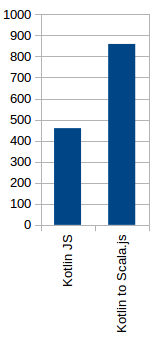
\includegraphics[height=8cm]{imgs/deltablue_barchart.png}
        \caption{DeltaBlue}
    \end{subfigure}
    ~
    \begin{subfigure}[h]{0.30\textwidth}
        \centering
        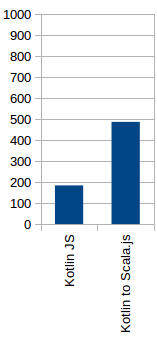
\includegraphics[height=8cm]{imgs/richards_barchart_firefox.png}
        \caption{Richards}
    \end{subfigure}
    ~
    \begin{subfigure}[h]{0.30\textwidth}
        \centering
        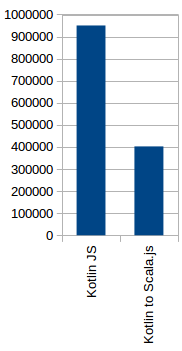
\includegraphics[height=8cm]{imgs/sha512_barchart_firefox.png}
        \caption{SHA512}
    \end{subfigure}
    \endgroup
  }
    
    \caption{Results in Firefox (lower is better)}
    \label{chart_firefox}
\end{figure*}


\begin{figure*}[h]
    \centering
    
  \resizebox{0.9\textwidth}{!}{
    \begingroup
    \begin{subfigure}[h]{0.30\textwidth}
        \centering
        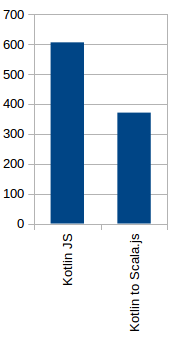
\includegraphics[height=8cm]{imgs/deltablue_barchart_chrome.png}
        \caption{DeltaBlue}
    \end{subfigure}
    ~
    \begin{subfigure}[h]{0.30\textwidth}
        \centering
        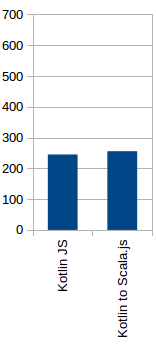
\includegraphics[height=8cm]{imgs/richards_barchart_chrome.png}
        \caption{Richards}
    \end{subfigure}
    ~
    \begin{subfigure}[h]{0.30\textwidth}
        \centering
        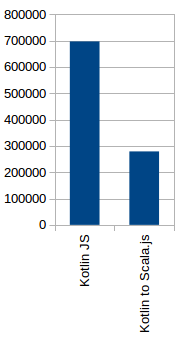
\includegraphics[height=8cm]{imgs/sha512_barchart_chrome.png}
        \caption{SHA512}
    \end{subfigure}
    \endgroup
  }
    
    \caption{Results in Google Chrome (lower is better)}
    \label{chart_chrome}
\end{figure*}


\begin{table}[htb]
  \centering
  \resizebox{\textwidth}{!}{
    \begingroup
    \renewcommand{\arraystretch}{1.5} % Default value: 1
    \begin{tabular}[c]{l | S[table-format=7.6] | S[table-format=4.6] | S[table-format=7.6] | S[table-format=5.6] |}
    & \multicolumn{2}{c|}{Kotlin JS} & \multicolumn{2}{c|}{Kotlin to Scala.js} \\ \hline
    
    Benchmark & \multicolumn{1}{c|}{Time ({$\mu$s})} & \multicolumn{1}{c|}{SEM} & \multicolumn{1}{c|}{Time ({$\mu$s})} & \multicolumn{1}{c|}{SEM} \\ \hline
    
    DeltaBlue & 459.28910 & 2.21871  & 859.11747 & 3.20804 \\
    
    LongMicro & & & & \\
    \multicolumn{1}{r|}{(LongNop)}    &   125.47639   &   0.70188 &   11.38803    &   0.02159 \\
    \multicolumn{1}{r|}{LongXor}    &   21.11297    &   0.77003 &   162.37052   &   0.56607 \\
    \multicolumn{1}{r|}{LongAdd}    &   165.33656   &   1.34534 &   198.32548   &   0.77713 \\
    \multicolumn{1}{r|}{LongMul}    &   2561.95739  &   4.75200 &   204.07814   &   0.63472 \\
    \multicolumn{1}{r|}{LongDiv32\_32}   &   6073.69372  &   28.94078    &   466.43548   &   1.08056 \\
    \multicolumn{1}{r|}{LongDiv32\_8}    &   8963.97814  &   14.92287    &   463.96042   &   1.00694 \\
    \multicolumn{1}{r|}{LongDiv53\_53}   &   5985.07349  &   26.34428    &   596.05268   &   1.27355 \\
    \multicolumn{1}{r|}{LongDiv53\_8}    &   9156.00966  &   72.35738    &   614.25587   &   1.59974 \\
    \multicolumn{1}{r|}{LongDiv64\_Pow2} &   9429.55544  &   18.06975    &   575.88860   &   1.01434 \\
    \multicolumn{1}{r|}{LongDiv64\_64}   &   5813.33312  &   13.79045    &   1028.32069  &   1.73338 \\
    \multicolumn{1}{r|}{LongDiv64\_8}    &   17033.25923 &   21.18046    &   1424.53345  &   2.37006 \\
    \multicolumn{1}{r|}{LongToString32} &   17519.93536 &   151.22958   &   552.06308   &   1.35633 \\
    \multicolumn{1}{r|}{LongToString53} &   28489.95217 &   250.54157   &   756.90514   &   5.21576 \\
    \multicolumn{1}{r|}{LongToString64} &   40159.85693 &   351.84462   &   3999.46757  &   33.08056    \\
    
    Richards & 184.11963 & 0.30823  & 487.24435 & 1.09796  \\
    SHA512 & 950152.00000 & 4554.93841 & 402408 & 8219.83114 \\
    \end{tabular}
    \endgroup
  }
  \caption{Results obtained in Firefox for both compilers}
  \label{raw_firefox}
\end{table}

\begin{table}[htb]
  \centering
  \resizebox{\textwidth}{!}{
    \begingroup
    \renewcommand{\arraystretch}{1.5} % Default value: 1
    \begin{tabular}[c]{l | S[table-format=7.6] | S[table-format=4.6] | S[table-format=7.6] | S[table-format=5.6] |}
    & \multicolumn{2}{c|}{Kotlin JS} & \multicolumn{2}{c|}{Kotlin to Scala.js} \\ \hline
    
    Benchmark & \multicolumn{1}{c|}{Time ({$\mu$s})} & \multicolumn{1}{c|}{SEM} & \multicolumn{1}{c|}{Time ({$\mu$s})} & \multicolumn{1}{c|}{SEM} \\ \hline
    
    DeltaBlue & 606.05524 & 1.78070 & 370.94092 & 1.52064 \\
    LongMicro & & & & \\
    \multicolumn{1}{r|}{(LongNop)}    &   95.09802    &   0.47985 &   43.68818    &   0.03876 \\
    \multicolumn{1}{r|}{LongXor}    &   154.29454   &   1.60520 &   132.63678   &   1.04405 \\
    \multicolumn{1}{r|}{LongAdd}    &   127.47245   &   1.58866 &   230.62637   &   2.32570 \\
    \multicolumn{1}{r|}{LongMul}    &   1061.11579  &   7.45646 &   228.63878   &   2.21889 \\
    \multicolumn{1}{r|}{LongDiv32\_32}   &   2808.60478  &   16.70720    &   462.99540   &   3.33924 \\
    \multicolumn{1}{r|}{LongDiv32\_8}    &   4144.76779  &   29.60327    &   445.63578   &   3.15253 \\
    \multicolumn{1}{r|}{LongDiv53\_53}   &   2704.16434  &   19.20949    &   513.25610   &   3.33351 \\
    \multicolumn{1}{r|}{LongDiv53\_8}    &   4481.03002  &   41.38667    &   499.07308   &   3.49403 \\
    \multicolumn{1}{r|}{LongDiv64\_Pow2} &   5165.94583  &   42.55326    &   490.20881   &   3.79047 \\
    \multicolumn{1}{r|}{LongDiv64\_64}   &   2804.60700  &   18.10513    &   849.86173   &   5.54424 \\
    \multicolumn{1}{r|}{LongDiv64\_8}    &   8631.07929  &   73.32333    &   1366.56581  &   6.29874 \\
    \multicolumn{1}{r|}{LongToString32} &   8129.34032  &   47.13448    &   504.82060   &   4.37917 \\
    \multicolumn{1}{r|}{LongToString53} &   13103.23530 &   93.32371    &   685.87353   &   6.50972 \\
    \multicolumn{1}{r|}{LongToString64} &   17988.75739 &   128.04266   &   1680.24284  &   8.84513 \\
	    
    Richards & 245.06567 & 0.49429 & 255.69825 & 0.52048 \\
	    
    SHA512 & 696866.00000 & 4694.32114 & 279157.5 & 11230.01427
    \end{tabular}
    \endgroup
  }
  
  \caption{Results obtained in Google Chrome for both compilers}
  \label{raw_chrome}
\end{table}

\begin{comment}
\paragraph{} As can be easily seen, the size of all output JavaScript code by the Kotlin to 
Scala.js compiler is significantly smaller. The major difference is due to the inclusion of the 
full Kotlin JS standard library with the generated code.
\end{comment}

\paragraph{} The results for the DeltaBlue benchmark are interesting. It seems that the implementation of the JavaScript runtime in both browsers differs at some point, leading Kotlin JS to perform better in Firefox whereas the Kotlin to Scala.js compiler has much better results in Google Chrome. It is hard to conclude which of the two compilers performed better here.

\paragraph{} Regarding the Richards benchmark, we can see that in Firefox Kotlin JS does better. This is probably because of the difference of translation of arrays between the two compilers. Scala.js keeps close to the JVM implementation of arrays and wraps all of them inside JavaScript classes. This requires a function call before obtaining the array itself and introduces execution overheads. This behavior allows to keep typing informations in the JavaScript code. Kotlin doesn't do that and therefore wins thanks to an implementation of arrays closer to JavaScript semantics.

\paragraph{} On the other hand, the execution times in Google Chrome are much closer. It is likely that this is of the same origin as for the DeltaBlue benchmark because of the indirection on array accesses.

\paragraph{} Both LongMicro and SHA512 benchmarks perform better with the Kotlin to Scala.js compiler in both web browsers. This large difference in performance is due to the optimized implementation of Longs in the Scala.js library and optimizer.



\chapter{Conclusion}
  \section{Project conclusion}
  \paragraph{} This project was (at first) aimed to finish the compilation of the Kotlin JS standard library in order to provide full support of the Kotlin features with the Kotlin to Scala.js compiler. Sadly, more features than expected were missing and a few still are, preventing a complete compilation. The range of unsupported language features has however been greatly reduced and one should easily be able to implement the last missing features.
  
  \paragraph{} The complete compilation of the standard library is slowed down as well by the need to write translation for uses of the Kotlin \ktinline{js} function.
  
  \paragraph{} Prior work on the compiler allowed to show that the use of the Scala.js linker for compiling Kotlin to JavaScript would lead to a huge improvement in terms of the size of the final JavaScript code emitted. This project shows that the performance of the Kotlin to Scala.js compiler still has room for improvement in some cases, mainly in the handling of array accesses. As for the other benchmarking results, this compiler is at least as good as what the Kotlin JS compiler would do and even much better in handling 64 bits integer operations.
  
  \paragraph{} The current state of the compiler is not suited for large scale projects but could however already be used for smaller sized applications. The fact that the Gradle plugin is fairly easy to configure removes the hard work required to satisfy the compilation pipeline since it doesn't require to operate things manually anymore.
  
  \section{Future work}
   
  \paragraph{} The current version of the compiler is still missing important features. In order to complete full classes support, data classes and inner classes must be supported. Destructuring declarations are also missing but can be really handy. They allow, for instance, to retrieve in one line the content of a method returning a tuple.
  
  \paragraph{} A strong improvement would be to provide a good algorithm for generating fresh names. As of now the utility function used throughout the project uses the generation of a unique identifier with the help of the UUID package from Java. This works but is however not a recommended way of doing this. This problem could be solved by adding the maintenance of a context which could be passed down to lower layers. Kotlin is already providing such a context but the way it is maintained in the Kotlin compiler is quiet unclear.
  
  \paragraph{} The main bottleneck for the use of the compiler is the fact that external classes and dynamic types are not well supported. Such an addition would allow for easy interaction with JavaScript existing features and provide access to the HTML DOM of web pages.
  

\begin{comment}
- Upgrade to 1.0.0-M1 (then M2)
- Is operator
- This keyword
- Binary operations
- Backing field + field keyword
- getters and setters with body
- kotlin js function support
- lambda expressions
- interfaces
- enum classes

- gradle plugin (tooling)

\end{comment}

\appendix

\include{utils}

\include{glossary}

\include{kotlin_stdlib}

\begin{comment}
  - brief explanation of the various utils available
  - definition of dispatch receiver, extension receiver
  - kotlin standard library compilation (which files and how)
\end{comment}


\nocite{*}
\bibliographystyle{apa}
\bibliography{mybib}{}

\end{document}